%% OJEPN context IBRE article
%% Licence: Creative Commons Attribution Share-Alike 4.0
%% Author:  Angus Inkster
%% Adapted from a creative commons template by Andy J. Wills

\documentclass[twocolumn]{article}
\usepackage[utf8]{inputenc}
\usepackage[T1]{fontenc}
\usepackage[english]{babel}
\usepackage{ifpdf,amsmath,amsthm,amssymb,amsfonts,newtxtext,newtxmath,xcolor} 
\usepackage{array,graphicx,dcolumn,multirow,hevea,abstract,hanging}
\usepackage{bm,multirow}
\usepackage[labelfont=sc,textfont=sf]{caption}
\usepackage[colorlinks=true,linkcolor=black,anchorcolor=black,citecolor=black,filecolor=black,menucolor=black,runcolor=black,urlcolor=black,hyperfootnotes=false,breaklinks=true]{hyperref}
\urlstyle{same}
\usepackage[hyphenbreaks]{breakurl}
\usepackage[natbibapa]{apacite}
%\usepackage{natbib} % must come afer hyperfootnotes
%\setlength{\bibsep}{0pt}
\usepackage{booktabs} % \toprule \midrule \bottomrule \cmidrule(lr){a-b}
% define centered and ragged columns:
\newcolumntype{L}[1]{>{\raggedright\arraybackslash }p{#1}} % can use m{}
\newcolumntype{C}[1]{>{\centering\arraybackslash }p{#1}}
\newcolumntype{R}[1]{>{\raggedleft\arraybackslash }p{#1}}
\newcolumntype{d}[1]{D{.}{.}{#1}} % d{3.2} for 3 places on l, 2 on r
\newcommand{\mc}{\multicolumn}
\topmargin=-.3in \oddsidemargin=-.1in \evensidemargin=-.1in \textheight=9in \textwidth=6.8in
\setlength\tabcolsep{1mm}
\setlength\columnsep{5mm}
\setlength\abovecaptionskip{1ex}
\setlength\belowcaptionskip{.5ex}
\setlength\belowbottomsep{.3ex}
\setlength\lightrulewidth{.04em}
\renewcommand\arraystretch{1.2}
\renewcommand{\topfraction}{1}
\renewcommand{\textfraction}{0}
\renewcommand{\floatpagefraction}{.9}
% \renewcommand{\baselinestretch}{1.00} \large\normalsize % for fixing spaces
\widowpenalty=1000
\clubpenalty=1000
\setlength{\parskip}{0ex}
\let\tempone\itemize
\let\temptwo\enditemize
\let\tempthree\enumerate
\let\tempfour\endenumerate
\renewenvironment{itemize}{\tempone\setlength{\itemsep}{0pt}}{\temptwo}
\renewenvironment{enumerate}{\tempthree\setlength{\itemsep}{0pt}}{\tempfour}

%%%%%%%%%%%%%%%%%%%%%%%%%%%%%%%%%%%%%%%%%%%%%%%%%%%%%%%%%%%%%%%%%%%%%
\setcounter{page}{22} % start with first page

\title{Effect of a context shift on the inverse base-rate effect}

\author{
	Angus B. Inkster\thanks{School of Psychology, Plymouth University, U.K.} 
	\and 
	Chris J. Mitchell\footnotemark[1] 
	\and
	René Schlegelmilch\thanks{Department of Psychology, University of Bremen.}
	\and
	Andy J. Wills\footnotemark[1] \hspace{0.01cm} \thanks{Email: andy@willslab.co.uk}  
}	

\date{} % leave empty
\begin{document} % goes here

% fill in short title
\newcommand{\jhead}{Open Journal of Experimental Psychology and Neuroscience, 2022}
\newcommand{\jdate}{Vol.~1}
\pagestyle{myheadings} \markright{\protect\small \jhead, \jdate \hfill CONTEXT AND THE IBRE \qquad}
\begin{htmlonly}
\end{htmlonly}
%\begin{latexonly}
\twocolumn[
\vspace{-.3in}
{\small \jhead, \jdate, 22--29  \hfill \url{https://doi.org/10.46221/ojepn.2022.0404}}
%\end{latexonly}

\maketitle

%\begin{latexonly}
\vspace{-3mm}
\begin{onecolabstract}
%\end{latexonly}

The Inverse Base Rate Effect (IBRE) is a non-rational behavioural phenomenon in predictive learning. In the IBRE, participants learn that a stimulus compound AB leads to one outcome and that another compound AC leads to a different outcome. Importantly, AB and its outcome are presented three times as often as AC (and its outcome). On test, when asked which outcome to expect on presentation of the novel compound BC, participants preferentially select the rarer outcome, previously associated with AC. This is irrational because, objectively, the common outcome is more likely. Usually, the IBRE is attributed to greater attention paid to cue C than to cue B, and so is an excellent test for attentional learning models. The current experiment tested a simple account of attentional learning proposed by \cite{LePelley2016} where attention paid to a stimulus is determined by its associative strength. This account struggles to capture the IBRE, but a potential solution presented by \cite{LePelley2016} appeals to the role of experimental context. In the present paper, we derived four predictions from the context explanation concerning the effect of changing to a novel experimental context at test, and examined these predictions empirically. Only one of the predictions, concerning the effect of a context shift on responding to a novel cue, was supported. These results fail to support both the context explanation suggested by \cite{LePelley2016} and the current leading account of the IBRE, EXIT (Kruschke, 2001b), but provide avenues for further research.

\smallskip
\noindent
Keywords: Inverse base-rate effect, EXIT, predictive learning, categorization
%\begin{latexonly}
\end{onecolabstract}\bigskip
]
%\end{latexonly}

{\renewcommand{\thefootnote}{}
\footnotetext{ % note blank lines above and below acknowledgment

\textbf{Author contribution statement}: ABI collected, analysed and interpreted the data, and led the writeup. CJM advised on the experimental design and on the writeup of the original submission. RS made significant contributions to the simulation work. AJW advised on the experimental design, analysis, and simulations, and co-wrote the article.
  
This experiment was funded by a full Ph.D. scholarship from Plymouth University to
the first author, and was reported as Experiment 4 in his thesis. The authors wish to thank Gemma Williams for helping to prepare some of the experimental materials, as part of an undergraduate research placement scheme at Plymouth University.

Copyright: \copyright\ 2022.
The authors license this article under the terms of the
\href{http://creativecommons.org/licenses/by/3.0/}{Creative Commons
  Attribution Share-Alike 4.0 License.}
}}

\saythanks

\setlength{\baselineskip}{12pt plus.2pt}

\section{Introduction}

The Inverse Base Rate Effect \cite[IBRE;][]{Medin1988} is a non-rational learning phenomenon that has generated considerable debate within the literature \citep{Kruschke1996a, Kruschke2001b, Juslin2001, Kruschke2003, Winman2003, Bohil2005, Don2021}. In its canonical form, participants are asked to diagnose fictitious patients under a simulated medical diagnosis procedure. They are initially presented with a patient showing one of two different symptom pairs, which can be considered abstractly as AB and AC. They are then asked to decide which of two fictitious diseases that patient has. For example, a participant might be presented with a patient suffering from a rash and nausea (AB), where the correct diagnosis is Jominy Fever. Then they might see a patient suffering from  a rash and back pain (AC), where the correct diagnosis is Phipps Syndrome. In this example nausea (B) is perfectly predictive of Jominy Fever, while back pain (C) is perfectly predictive of Phipps Syndrome. The rash (A) is uninformative. Participants see patients for whom the correct diagnosis is Jominy Fever three times as often as those for whom the correct diagnosis is Phipps Syndrome. In other words, Jominy Fever is a common disease, while  Phipps Syndrome is a rare disease. Participants are then presented with both perfectly predictive symptoms together, nausea (B) and back pain (C). If participants correctly make use of the base rate of the two diseases, they should make the rational diagnosis of the more common disease (Jominy Fever in our example). However, the majority of participants preferentially diagnose the patient with the rarer disease. This pattern of responding is called the IBRE.

The IBRE sometimes co-occurs with another response pattern. Specifically, common-disease responding to B is sometimes observed to be greater than rare-disease responding to C, when these stimuli are presented individually at test. This is surprising; it suggests that B is more strongly associated with the common outcome than C is with the rare outcome, while C dominates responding when they are presented in conjunction. This response pattern has been reported in a number of studies \citep[e.g.][]{Bohil2005, Winman2005}, with \cite{Wills2014} first confirming that the difference was statistically significant; a finding that has recently been replicated by \cite[Exp.~3]{Inkster2019}. We refer to the co-occurrence of the IBRE and this response pattern as the COmpound versus FEatures Dissociation (COFED). We describe the effect as a dissociation because the response to the compound BC is opposite to what one would expect from the summation of the responses to the individual cues. 

% AI: I took the reference to the HBM paper out of the above paragraph. I checked the DAU and whilst its numerically in the right direction, it's not significant (p = 0.16).

\begin{figure}[t]
	\centering
	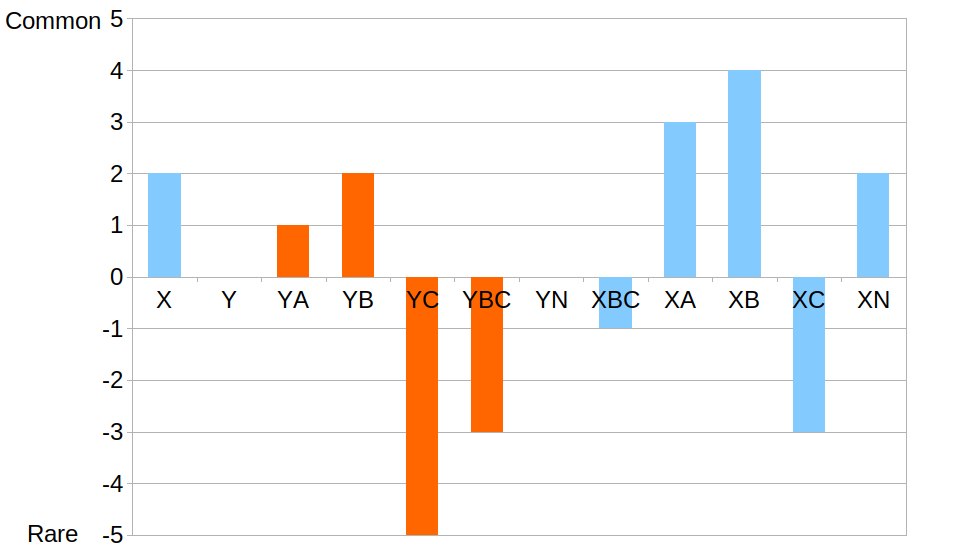
\includegraphics[width = .49\textwidth,trim = 0cm 0cm 0cm  0cm,clip]{cstims.png}
	\caption{Informal example of the context explanation of the COFED. Blue bars represent associative strengths for stimuli where the training context cue (X) is present. Orange bars represent associative strengths for cues where a novel context cue (Y) is present. The values on the y-axis represent arbitrary associative weights for the two outcomes.}
	\label{cstims}
\end{figure}

Although several potential explanations of the IBRE and the COFED exist, the EXIT model \citep{Kruschke2001a} is a strong contender. EXIT has previously accounted for the IBRE \citep{Kruschke2001a,Kruschke2005a} and the COFED \citep{Kruschke2003}, although it is worth noting that in the latter paper, this was after more heavily weighting the B vs C difference than other response patterns in the model fits. EXIT assumes that the IBRE is driven by an error-driven learning attentional effect, where the participant learns to direct their attention away from cues that lead to prediction errors. Specifically, early in training, participants make many errors on rare AC trials due to their similarity to common AB trials. EXIT assumes that people learn to avoid those errors by directing their attention on AC trials away from A and towards C. This trial-to-trial attentional shifting leads to the C cue dominating responding when presented with BC. Unlike earlier accounts of the IBRE by Kruschke, attention is assumed to be persistent, such that the IBRE occurs even in cases where B is more strongly associated to the common outcome than C is to the rare outcome (a COFED).

Recently, \cite{LePelley2016} argued that much of the data relating to human attentional learning could be {ccounted for by a simpler model than EXIT and its relatives \citep[e.g.][]{Mackintosh1975}. In this model, the attention that a stimulus demands is a simple function of the associative strength of that stimulus. Although consistent with much of the attentional learning literature, this simple model appears to be undermined by the IBRE; here, the cue that appears to possess the greatest associative strength (B) does not attract more attention than the weaker cue (C). \cite{LePelley2016} published\footnote{The idea was suggested in an unpublished peer review of this paper by Evan Livesey.} a potential solution to this, appealing to the role of experimental context.  Experimental context refers to the procedural context of the experiment. In a medical diagnosis task, examples of experimental context include the patients being diagnosed or where patients are diagnosed.

In this context explanation, the experimental context is represented as a cue that is present on every trial; cue X. In the IBRE procedure, X becomes more strongly associated with the common outcome (also associated with B) than the rare outcome (also associated with C), due to the greater frequency of the common outcome. Figure \ref{cstims} illustrates how the COFED can be explained from this assumption, plus the assumption that the associative strength from C to the rare outcome is greater than the associative strength from B to the common outcome (we leave aside the issue of why C might have greater associative strength than B at this point). In the context account, responding to cue compounds at test is then predicted by summing the associative strengths of the cues they contain. As can be observed in Figure \ref{cstims}, XBC results in rare responding (an IBRE), while at the same time there is more common responding to XB than there is rare responding to XC (a COFED). 

This context account of the IBRE and COFED leads to four predictions concerning  switching to a novel context (Y) at test. The first prediction is that YBC produces a larger proportion of rare responding than XBC---in other words, a context shift should enhance the size of the IBRE due to the novel context having no association to either outcome. The second prediction is that rare responding to YC will be greater than common responding to YB---a context shift will reverse the COFED. The third prediction is that while a novel cue presented in the same context as training (XN) should produce common responding, a novel cue presented in a novel context (YN) should not produce preferential responding to either the common or the rare outcome. In other words, a shift to context Y will bias responding away from the common outcome (with which context X is associated) and towards the rare outcome. The fourth prediction is that YA produces a lower proportion of common responding than XA ---in other words, a context shift should reduce the size of the common preference for A. These predictions are illustrated in Figure \ref{cstims} as the orange bars.

Previous evidence against the first prediction of the context account comes from the work of Don and colleagues \citep{Don2017, Don2019}. In these studies, overall outcome frequency was balanced while maintaining the other elements of the IBRE design, effectively removing any influence context might have on responding. This led to a reduced rare-outcome bias for BC, rather than the increase that the context account would have predicted. However, these previous experiments also provide evidence supporting the fourth prediction of the context account, which predicts reduced common-outcome responding to the imperfect cue (A); this is observed by both \cite{Don2017} and \cite{Don2019}. Unfortunately, these studies do not permit a direct assessment of the other two predictions of the context account. The effect of context on the COFED cannot be assessed, because no COFED is observed in the Standard conditions of these experiments. The effect of context on a novel cue also cannot be directly assessed from these previous studies, as in those studies the novel cue (N) was presented in compound with the imperfect predictor (A). Hence, the effect observed on the novel test compound (AN) may be due to the effects of context on the imperfect predictor, rather than the effects of the context on the novel cue.\footnote{This should not be construed as a criticism of Don and colleagues, who had other reasons for being interested in the AN compound.} In the experiment we report below, we directly test all four predictions of the context account. 

\section{Method}

\subsection{Participants}

Participants were all undergraduate students from the University of Plymouth, completing the experiment for partial course credit. Ninety four participants were tested. Assuming participant exclusion rates similar to \cite{Inkster2019}, this sample size provides adequate power to detect a small-to-medium-sized effect of context shift ($d = .31$ at 80\% power). It further provides over 99\% power to detect the IBRE and the COFED, at the effect sizes observed in \cite{Inkster2019}, $d = .46$ and $.56$, respectively.

\begin{table}[t]
	\caption{Abstract trial types for the training and test phases of the experiment. Bold type highlights the test stimuli of primary theoretical interest. The training trials also appear in the test phase and participants continue to receive feedback at test for these trials to maintain learning.}
	\begin{tabular}{L{1.4in}L{1.4 in}C{.2in}}\toprule
		Training trials (relative frequency) & Test trials & \\\midrule
		$A_{1}B_{1} \to common$ (x 2) & $A_{1}B_{1},A_{2}B_{2},A_{3}B_{3},$ & \\ 
		$A_{2}B_{2} \to common$ (x 2) & $F_{1}D_{1},F_{2}D_{2},F_{3}D_{3},$ & \multirow{ 2}{*}{x 2}\\
		$A_{3}B_{3} \to common$ (x 2) & $\bm{B_{1}},\bm{B_{2}},\bm{B_{3}},\bm{C_{1}},\bm{C_{2}},\bm{C_{3}},$& \\ 
		$A_{1}C_{1} \to rare$ (x 1) & $D_{1},D_{2},D_{3},E_{1},E_{2},E_{3}$
		& \\
		\cline{2-2}
		$A_{2}C_{2} \to rare$ (x 1) & $A_{1}C_{1},A_{2}C_{2},A_{3}C_{3},$ & \\
		$A_{3}C_{3} \to rare$ (x 1) & $G_{1}E_{1},G_{2}E_{2},G_{3}E_{3},$ & \\
		$F_{1}D_{1} \to common$ (x 2) & $\bm{B_{1}C_{1}},\bm{B_{2}C_{2}},\bm{B_{3}C_{3}},$ & \multirow{ 2}{*}{x 1} \\
		$F_{2}D_{2} \to common$ (x 2) & $D_{1}E_{1},D_{2}E_{2},D_{3}E_{3,}$ & \\
		$F_{3}D_{3} \to common$ (x 2) & $A_{1},A_{2},A_{3},$ & \\
		$G_{1}E_{1} \to rare$ (x 1) & $\bm{N_{1|4}},\bm{N_{2|5}},\bm{N_{3|6}}$ & \\
		$G_{2}E_{2} \to rare$ (x 1) & & \\
		$G_{3}E_{3} \to rare$ (x 1) & & \\
	\end{tabular}
	\label{exp1trn}	
\end{table}

\subsection{Stimuli and apparatus}

The stimuli (see Figure~\ref{cellexample}) were abstract shapes, red and yellow in colour and 30 x 30 pixels in size; previously used in \cite{Wills2014}. They were displayed on 22-inch flat-screen monitors using PsychoPy \citep{Peirce2007}. Participants sat approximately 50 cm from the screen, giving each cell a visual angle of approximately 2 degrees. Responses were collected using a standard PC keyboard.

\begin{figure}[b]
	\centering
	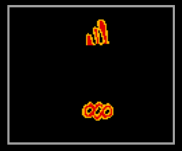
\includegraphics[width = .25\textwidth]{exp1trnclose.png}
	\caption[Example trial]{An example compound stimulus.}
	\label{cellexample}
\end{figure}

Table \ref{exp1trn} shows the combinations of abstract cues and diseases presented in the training and test phases of the experiment. The stimuli were assigned at random to one of 7 abstract cues (A-G) for each participant for the training phase. As in \cite{Wills2014}, each abstract cue had 3 stimuli assigned to it. A subset of possible cell combinations was used for the compound cue trials, for example on AB trials the cells presented were: $A_{1}B_{1}$, $A_{2}B_{2}$ or $A_{3}B_{3}$. The cue compounds FD and GE represent disjoint cue trials, where the proportion of outcomes is the same as AB and AC but there is no shared cue. During the test phase one more abstract cue was presented, the novel cue, N. N had six stimuli assigned to it, rather than the three assigned to the other abstract cues. This is due to the novel nature of the cue and the fact that there are two test phases; resulting in three of the cues assigned to N being used in the first test phase and the other three in the second. In total, 27 different cells were used in this experiment. Two diseases were used as outcomes: ``Jominy Fever'' and ``Phipps Syndrome''. Diseases were mapped to the abstract disease types in both possible ways, across participants, as were the response keys mapped to those diseases.

\subsection{Procedure}

The procedure was closely based on \cite{Wills2014}, with the addition of a context manipulation. Participants were tasked with diagnosing patients with one of two diseases, Jominy Fever or Phipps Syndrome, on the basis of the ``cells'' they were presented with. Two contexts were used, one where participants diagnosed human patients and one where they diagnosed orcs. Participants always diagnosed humans during training, but completed two test phases, one with orcs and one with humans. The order of the test phases was counterbalanced between participants. In each of the three phases (one training, two test) the trial order was randomised between participants.

The training phase comprised 20 blocks of 18 trials, 360 trials in total. Each trial began with a 1000 ms presentation of a grey viewbox, which indicated where the cells would appear. The cells then appeared, centralised horizontally, but towards the top and bottom of the viewbox vertically. The cell presented to the top and to the bottom of the view box was randomised on each trial. The cells remained on screen for a maximum of 2000 ms, during which time participants made their diagnosis using the ``c'' and ``m'' keys. Once a response was made, the cells disappeared and participants received feedback, telling them if they were right or wrong and what the correct diagnosis was. Feedback was presented on screen for 1500 ms before a new trial began. If a response was not made during the 2000 ms the cells were on screen, participants instead received a time-out message, displayed for the same duration as the feedback. 

In the ``orcs'' test phase, participants were told they would be completing a medical placement in a different dimension and would now be diagnosing orcs. This was further emphasized on every trial by surrounding the viewbox with a large green outline of an orc's face. In the ``humans'' test phase, participants were told they would continue to diagnose humans. Each test phase consisted of 216 trials, with the same trial structure as in the training phase, and single cells being presented in the middle of the viewbox. Feedback continued to be presented for stimuli that were presented during the training phase, in order to maintain learning. For the novel cues and compounds, no feedback was presented; participants instead received the message ``data missing''. Time-out messages continued to be displayed if a response was not made in 2000ms. 

\section{Results}

Raw data, analysis and modelling scripts are available at \url{https://osf.io/8p42b/}. Analysis was conducted using R \citep{R2018}, with packages, \emph{ez} \citep{ez2016}, \emph{tidyr} \citep{tidyr2019}, \emph{dplyr} \citep{dplyr2019},and \emph{pwr} \citep{pwr2018}. Null-hypothesis significance tests were conducted at an alpha level of .05.\footnote{Exact p-values, i.e. $P(data|H_{0})$, are included at the request of a reviewer.}

Bayesian tests were also conducted, with Bayes Factors less than one third interpreted as substantial evidence for the null, and Bayes Factors greater than 3 were interpreted as substantial evidence for the alternative. Where possible, prior effect sizes were drawn from previous related experiments reported in \cite{Inkster2019}. Following \cite{Dienes2011}, these effect sizes were used to construct a half-normal prior with a mean of zero and a standard deviation of the prior effect size. Where no relevant effect sizes were available we instead used an uninformative prior, ranging from the lowest to the highest possible group difference (the measures were proportions and hence had to fall between 0 and 1).\footnote{This analysis methodology enhances sensitivity, relative to analysis reported in the first author's unpublished thesis \citep{Inkster2019}.} 

Following \cite{Wills2014}, participants who did not score significantly above chance in the final block of training were excluded. Eighteen participants were excluded in this way; this rate of exclusion is slightly higher than \cite{Wills2014}, but similar to that reported by \cite{Inkster2019}. Trials where a timeout occurred for the remaining participants were removed from analysis and constituted less than 1\% of trials.

Accuracy across the training phase is shown in Figure \ref{exp1tacc}. In the final block of training, participants were more accurate on common-outcome trials (AB, FD) than rare-outcome trials (AC, GE), $F(1,75) = 51.02, p = 5.01 \text{x} 10^{-10}, f = .83$, and more accurate in the non-shared cue trials (FD, GE) than on shared cue trials (AB, AC), $F(1,75) = 26.72, p = 1.89 \text{x} 10^{-6}, f = .60$. The interaction  was also significant, $F(1,75) = 14.39, p = 2.99 \text{x} 10^{-4}, f = .44$. 

\begin{figure}[b!]
	\centering
	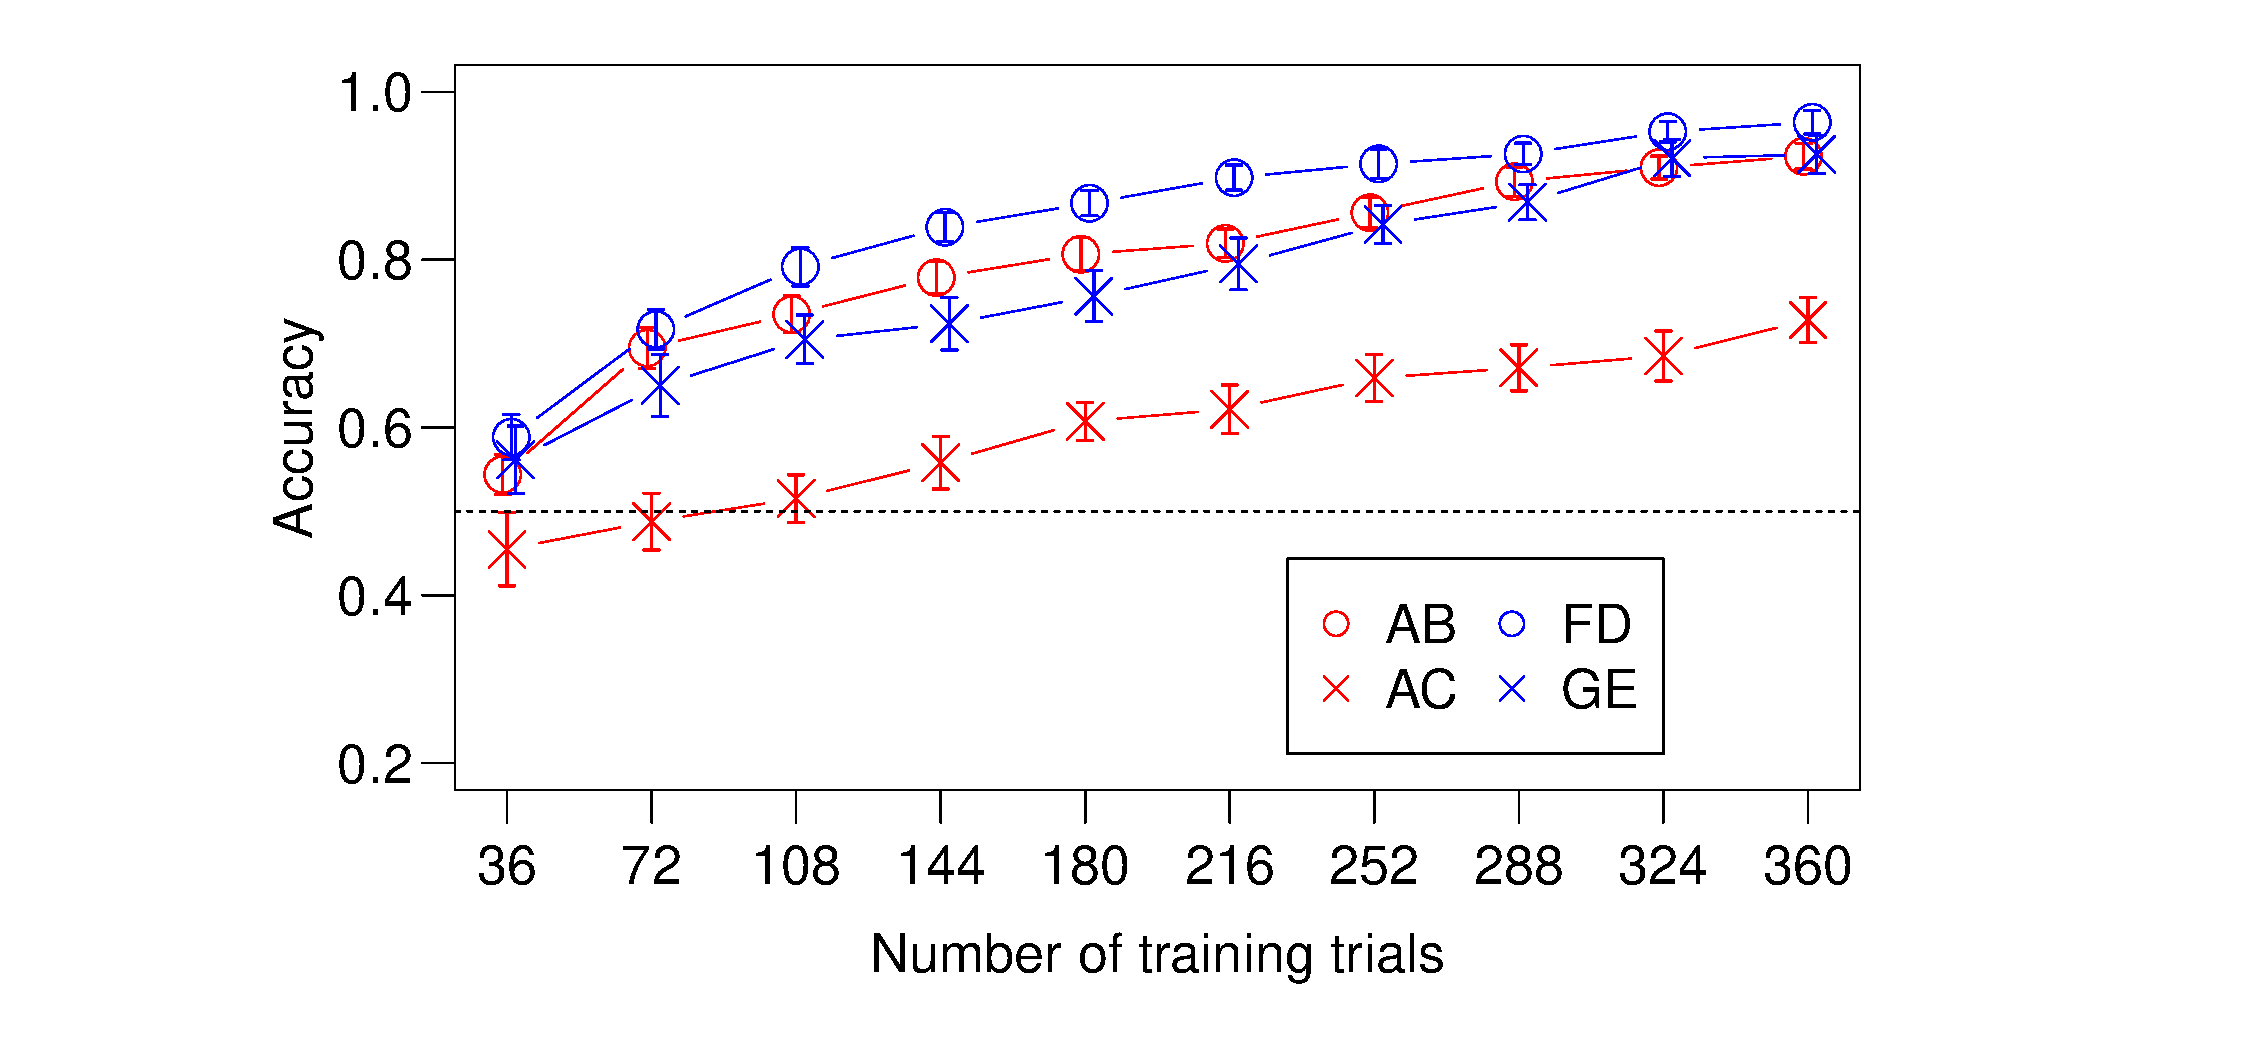
\includegraphics[width = .49\textwidth,trim = 4.5cm 1cm 6cm  1cm,clip]{exp1tacc.pdf}
	\caption[Training accuracy]{Participants' accuracy on the abstract training trial types at different levels of training. The error bars represent within-subject Cousineau-Morey 95\% confidence intervals}
	\label{exp1tacc}
\end{figure}

In the test phase, all participants received both a same-context test phase (humans), and a different-context test phase (orcs). In the following analyses, context (same vs. different) is treated as a within-subjects factor.\footnote{Analyzing the first test phase alone, employing context as a between-subjects factor, produces the same direction of results, but the analysis is less conclusive due to the reduced power of between-subject tests relative to within-subject tests.}  Table \ref{exp1testacc} shows the response proportions for each stimulus under both same-context and different-context conditions. Cues that are abstractly identical have been combined in this Table. For example, ``A'' represents responses to  $A_{1}$, $A_{2}$, and $A_{3}$. In the following analyses, the data were first analysed within the same and different conditions, and then between the two conditions. 

\begin{table}[t]
	\caption[Response proportions at test]{Proportion of \textit{common} and \textit{rare} responses to each of the stimulus types presented under different-context and same-context conditions. Bold type highlights the results of primary theoretical interest. Values within brackets represent response proportions from the simulation of this experiment using the EXIT model with optimised parameters.}
	\begin{center}
		\begin{tabular}{C{.9in} C{.5in} C{.5in} C{.5in} C{.5in} }\toprule
			\multicolumn{1}{c}{} & \multicolumn{2}{c}{\textit{Common}} & \multicolumn{2}{c}{\textit{Rare}} \\
			\cline{2-5}
			Stimulus type & Same & Diff & Same & Diff \\\midrule
			A & .72\it{(.74)} & .69\it{(.67)} & .28\it{(.26)} & .31\it{(.33)} \\
			AB & .89\it{(.89)} & .87\it{(.87)} & .11\it{(.11)} & .13\it{(.13)} \\
			AC & .30\it{(.27)} & .30\it{(.26)} & .70\it{(.73)} & .70\it{(.74)} \\
			B & \bf{.87}\it{(.88)} & \bf{.88}\it{(.86)} & .13\it{(.12)} & .12\it{(.14)} \\
			BC & .42\it{(.44)} & .42\it{(.43)} & \bf{.58}\it{(.56)} & \bf{.58}\it{(.57)} \\
			C & .26\it{(.21)} & .26\it{(.19)} & \bf{.74}\it{(.79)} & \bf{.74}\it{(.81)} \\
			D & .90\it{(.85)} & .88\it{(.83)} & .10\it{(.15)} & .12\it{(.17)} \\
			DE & .47\it{(.48)} & .47\it{(.47)} & .53\it{(.52)} & .53\it{(.53)} \\
			E & .25\it{(.28)} & .26\it{(.26)} & .75\it{(.72)} & .74\it{(.74)} \\
			FD & .94\it{(.92)} & .92\it{(.91)} & .06\it{(.08)} & .08\it{(.09)} \\
			GE & .14\it{(.18)} & .15\it{(.18)} & .86\it{(.82)} & .85\it{(.82)} \\
			N & \bf{.57}\it{(.52)} & \bf{.50}\it{(.50)} & .43\it{(.48)} & .50\it{(.50)} \\
		\end{tabular}
	\end{center}
	\label{exp1testacc}
\end{table}

\paragraph{Same-context  test.} The proportion of rare-outcome responding to BC was greater than .5, $t(75) = 2.82, p = .003, d = .32, BF_{10} = 21$, indicating the presence of an IBRE. Common-outcome responding to B was greater than rare-outcome responding to C, $t(75) = 4.87, p = 3.07 \text{x} 10^{-6}, d = .56, BF_{10} = 3.36 \text{x} 10^{4}$; together with the IBRE, this demonstrates the presence of the COFED in this condition. The proportion of common-outcome responses to the novel stimulus, N, was greater than .5, $t(75) = 2.11, p = .019, d = .24, BF_{10} = 3.66$. Similarly, the proportion of common-outcome responding to A was greater than .5, $t(75) = 9.32, p = 1.87 \text{x} 10^{-14}, d = 1.07, BF_{10} = 7.19 \text{x} 10^{17}$.

\paragraph{Different-context test.} The IBRE was again observed, $t(75) = 3.23, p = .002, d = .37, BF_{10} = 11$, as was greater common-outcome responding to B than rare-outcome responding to C, $t(75) = 5.25, p = 1.36 \text{x} 10^{-6}, d = .60, BF_{10} = 3.13 \text{x} 10^{4}$, again demonstrating the COFED. Common-outcome responding to N did not differ from .5, $t(75) = .1, p = .92, d = .01, BF_{10} = .09$. Common-outcome responding to A again was greater than .5, $t(75) = 8.29, p = 3.22 \text{x} 10^{-12}, d = .95, BF_{10} = 5.30 \text{x} 10^{13}$.

\paragraph{Effect of changing context.} The proportion of rare-outcome responding to BC, and hence the size of the IBRE, was unaffected by the change in context, with substantial evidence for the null, $t(75) = .31, p = .76, d = .03, BF_{10} = .03$. Similarly, neither common-outcome responding to B, nor rare-outcome responding to C, was affected, again with substantial evidence for the null; $t(75) = 1.02, p = .31, d = .12, BF_{10} = .02$ and $t(75) = .20, p = .84, d = .02, BF_{10} = .02$, respectively. Taken with the evidence suggesting that context shift has no effect on the IBRE, this suggests that context shift has no effect on the COFED. However, the change in context did reduce the proportion of common-outcome responding to N, $t(75) = 2.23, p = .014, d = .26, BF_{10} = 3.40$. Finally, common-outcome responding to A was unaffected by the change in context, with substantial evidence for the null, $t(75) = 1.26, p = .11, d = .14, BF_{10} = .05$.

\section{Discussion}

\subsection{Summary and interpretation of findings}

We observed both the inverse base-rate effect (IBRE) and the compound versus features dissociation (COFED) in this experiment, replicating the results of \cite{Wills2014} and \cite[Exp.~3]{Inkster2019} in this regard. However, the context-based explanation of the COFED published by \cite{LePelley2016} was largely not supported by the current experiment. First, the context explanation predicts an increase in the size of the IBRE with a change to a novel context at test, while in our experiment this had no effect, with Bayesian evidence for the null. Second, the context explanation predicted a reversal of the COFED with a change of context, while we observed no effect, again with Bayesian evidence for the null. Third, the context account predicted a reduction in common-outcome responding to the imperfect cue (A), which again was not observed, with Bayesian evidence for the null. However, fourth, it would be difficult to argue that the context manipulation went unnoticed by the participants, because it affected the proportion of common-outcome responding to a novel cue, in the manner predicted by the context account.

In fact, the context account can only predict the 50:50 responding we observed to the novel cue in the novel context  under the assumption that the change of context was essentially complete. Further, the context account predicts the same effect size for the one phenomenon we did observe, and the three we did not. For example, inspection of Figure 1 shows a effect size of 2 (arbitrary units) for both the novel cue (N), and the IBRE (BC). Thus, while it possible to imagine ways in which the two contexts of our experiment overlap, doing so does not explain the presence of one, but absence of three, equal-sized effects predicted by the context account. Overall, the context account does not provide a compelling explanation of our results.

\subsection{The EXIT model}

The best fit of the EXIT model to our data is shown in Table \ref{exp1testacc}; for technical details of our simulation methodology, see the Appendix. EXIT captures both responding to a novel cue and the effect of context shift on responding to a novel cue, effects that EXIT has not been tasked with capturing previously. Its ability to do this comes from the fact that EXIT (like the account published by \citeauthor{LePelley2016}) assumes that a context cue is present on every trial. This context cue becomes preferentially associated to the common outcome. On a novel-cue trial, the context is the only cue that has any associative strength, and so it is the only basis on which a prediction can be made. When the context changes, there is no basis within EXIT to make a prediction about the novel cue and so it responds randomly.

Although our EXIT simulation has acceptable quantitative fit to our data ($RMSD = .03$) it nonetheless suffers from much the same problems as the context account published by Le Pelley et al., and for much the same reasons. More specifically, although EXIT correctly predicts that (1) the change of context reduces the rate of common-outcome responding to N, it also incorrectly predicts that context shift should (2) reduce common-outcome responding to A, (3) reduce the extent to which $B > C$, and (4) reduce rare-outcome responding to BC. The size of the predicted effect in the case of predictions 2 and 3 is larger than the size of the predicted effect in prediction 1. Thus, EXIT predicts some things that are observed, but also predicts, more strongly, other things that aren't observed. Like the context account, it fails to provide a full explanation of our results. 

\subsection{Previous and future research}

\cite{Wills2014} previously reported preferentially common responding for cue compound DE, which was not observed in this experiment. This is the third time we have failed to replicate this particular aspect of our previous work under closely similar procedures; the other two were Experment 3 of \cite{Inkster2019}, and the experiment reported by \cite{Inkster2019c}. Thus, contrary to \cite{Wills2014}, it seems likely that DE does not produce preferentially common responding in this procedure. All other principal behaviours in the original study (i.e. the IBRE and the COFED) are observed across the original study and two replications in our lab.

The poor performance of participants on AC, relative to other IBRE procedures in the literature, is also characteristic of all four times we have run this procedure, and may be the cause of the COFED in our procedure. This is noteworthy because, although the COFED is consistently replicable within the procedures of the current experiment, it appears to be somewhat procedure dependent. Specifically, although we have now found a significant COFED on three separate occasions with the current procedure, changes in procedure can result in either an IBRE without a COFED (C greater than B, rather than B greater than C), or the B greater than C component of the COFED without the accompanying IBRE \citep{Inkster2019}. One possible explanation is that, with insufficient training, an IBRE is not observed but, with too much training, performance on both B and C are at ceiling, precluding the ability to observe a COFED. Thus, a COFED might only be observed where there is some learning of AC during training, but this learning is incomplete. This possibility merits further investigation.

A second possible topic for future research concerns the responding to a novel cue at test. In the current experiment, we reported common-outcome responding when the context was the same as in training. Interestingly, this result is in contrast to \cite{Juslin2001} who reported that, under some conditions, a novel cue receives preferentially rare-outcome responding. Two other studies of the IBRE have also presented a novel cue at test. \cite{Johansen2007} reported preferentially-rare responding, but did not statistically analyze those data, and used a procedure quite unlike those of other IBRE experiments, in that the training phase was presented to participants in summarised form. As discussed in the introduction, \cite{Don2017} reported preferentially-common responding under standard conditions when they presented the novel cue in compound with a familiar cue A. Further research into the conditions under which novel cues lead to common- or rare-outcome responding is merited. 

A third future research topic follows on from the comparison of our findings to those of \cite{Don2017} and \cite{Don2019}. In these previous studies, the authors noted a reduction in the strength of the IBRE after balancing outcome frequency and effectively removing context associations. Our experiment instead shifted context to achieve the same goal, but did not find the same reduction in rare responding to the IBRE, instead observing a reduction in common responding to a novel cue, which was only observed in Experiment 3 of \cite{Don2017}. Notably, \cite{Don2017} only found the $B > C$ response pattern in the absence of an IBRE, indicating the lack of a COFED. It's also the case that Don and colleagues found an effect of context on the imperfect cue A, while we did not. Further work investigating how and why these two approaches to removing context associations differ would be informative. One reasonable hypothesis on the basis of current data is that the effects of context on the IBRE depend on whether it is observed with or without a COFED.

Finally, in our experiment, the same-context test always uses human patients, while the different-context test is always orc patients. It is therefore possible, in principle, that the difference in novelty of these contexts in some way influenced our results. However, in the context of a task that involves diagnosing fictious diseases on the basis of a large number of abstract confusable shapes, we suspect novelty may be at ceiling for both contexts. Nonetheless, future research may wish to counterbalance the training context between participants. 



\subsection{Conclusion}

The current study of context manipulation in the IBRE raised some new questions for future research, but it also provided a clear answer to the question we set out to investigate. Specifically, our results largely do not support the context explanation of the IBRE and COFED published by \cite{LePelley2016}. Our results also seem problematic for EXIT \citep{Kruschke2001b}, the leading model of the IBRE; this is to be expected as the two accounts represent experimental context in much the same way. Thus, more than twenty years after the publication of the EXIT model, a fully adequate explanation of the IBRE remains elusive.

\setlength{\bibhang}{15pt}

\bibliographystyle{apacite}
%\bibpunct[ ]{(}{)}{;}{a}{}{,} 
\bibliography{references}


\section*{Appendix: Modelling}

These simulations were conducted using \emph{slpEXIT}, part of the \emph{catlearn} R package \citep{catlearn2019}. This implementation of EXIT is based on the model as described in \cite{Kruschke2001b}, with the inclusion of a bias cue that was later implemented in \cite{Kruschke2003}. The bias cue was assumed to be analogous to the experimental context in Le Pelley et al.'s explanation. As such, two bias cues were implemented, one for each context, with the salience of these cues represented by the $\sigma$ parameter. 

The EXIT model was applied to simulated training and test trials that replicated the details of experimental procedure, generating response patterns for each simulated trial. The values of the free parameters given to the model were varied using the \emph{optim} function in R \citep{R2018}. The goal of this variation was to optimise the free parameters given to the model; in order to find the parameter set that when given to the model gave the closest approximation to the behavioural data. This was accomplished by calculating the sum of squared errors (SSE) between the response patterns generated by the model under a specific parameter set and the behavioural response patterns; \emph{optim} was used to find the parameter set that minimised the SSE.

The method used for optimisation within optim was the limited memory Broyden-Fletcher-Goldfarb-Shanno (BFGS) algorithm \citep{Byrd1995}. As optim requires an initial set of parameters to vary, each free parameter within the EXIT model was initially set to one of two values. As there are 7 free parameters, this resulted in a total of $7^{2}$ or 128 sets of parameter values. Each of these starting parameter sets were supplied to optim individually. optim then used the BFGS algorithm to perform a hill-climbing optimisation and arrive at an optimised parameter set for each individual starting set. This produced 127 sets of optimised parameter values.\footnote{One starting parameter set failed to optimise. The final optimised set was drawn from the 127 sets that successfully optimised.} These sets of optimised parameters values were compared in terms of the SSE generated when they were given to EXIT, in order to identify the set that produced the lowest SSE. The parameter values within this final optimised set for the experiment we report were: $c = .399, P = 2.342, \phi = 3.729, \lambda_{g} = .348, \lambda_{w} = .023, \lambda_{x} = 2.901, \sigma = .008$.

\end{document}

%%% Local Variables:
%%% mode: latex
%%% TeX-master: t
%%% End:
